%%%%%%%%%%%%%%%%%%%%%%%%%%%%%%%%%%%%%%%%%
% FAIMS3 Presentations
% LaTeX Template
% Version 1.0 (May 1, 2021)
%
% This template was created by:
% Vel (enquiries@latextypesetting.com)
% https://www.LaTeXTypesetting.com
%
%!TEX program = xelatex
% Note: this template must be compiled with XeLaTeX rather than PDFLaTeX
% due to the custom fonts used. The line above should ensure this happens
% automatically, but if it doesn't, your LaTeX editor should have a simple toggle
% to switch to using XeLaTeX.
%
%%%%%%%%%%%%%%%%%%%%%%%%%%%%%%%%%%%%%%%%%

\documentclass[
	aspectratio=169, % Wide slides by default
	12pt, % Default font size
	t, % Top align all slide content
]{beamer}

\usetheme{faims} % Use the FAIMS beamer theme
\usecolortheme{faims} % Use the FAIMS beamer color theme

\bibliography{references.bib} % BibLaTeX bibliography file
\bibliography{faims-zotero-betterbibtex.bib}
%----------------------------------------------------------------------------------------

\begin{document}
\begin{refsegment}
%https://tex.stackexchange.com/a/19328
%https://tex.stackexchange.com/a/223074
%----------------------------------------------------------------------------------------
%	 TITLE SLIDE
%----------------------------------------------------------------------------------------


% \title{FAIMS 3.0: Electronic Field Notebooks} % Presentation title
% \author{S Ross, P Crook, B Ballsun-Stanton, S Cassidy, A Sobotkova, J Klump}   % Presentation author
% \institute{Australian Astronomical Optics seminar}   % Author affiliation
% \date{19 August 2021}    % Presentation date  


\begin{titleframe} % Custom environment required for the title slide
	\frametitle{FAIMS 3.0}
	\framesubtitle{Electronic Field Notebooks}

	S Ross, P Crook, B Ballsun-Stanton,\\ S Cassidy, A Sobotkova, J Klump

    \bigskip
	Australian Astronomical Optics seminar

	\vfill

	19 August 2021
\end{titleframe}

%----------------------------------------------------------------------------------------
%	TABLE OF CONTENTS
%----------------------------------------------------------------------------------------

% \begin{frame}
% 	\frametitle{Table of Contents}
% 	\framesubtitle{One Column}

% 	\tableofcontents % Sections are automatically populated from \section{} commands through the presentation
% \end{frame}

%------------------------------------------------

\begin{frame}
    \frametitle{Strategies for field data capture infrastructure}
	%\framesubtitle{Two Columns}
    
    \begin{columns}[t]
        \begin{column}{0.45\textwidth}
            \tableofcontents[sections={1-3}] % Sections are automatically populated from \section{} commands through the presentation
        \end{column}
        \hfill
        \begin{column}{0.45\textwidth}
            \tableofcontents[sections={4-6}] % Sections are automatically populated from \section{} commands through the presentation
        \end{column}
    \end{columns}
\end{frame}

%----------------------------------------------------------------------------------------

\section{`Small Data' Infrastructure}

\begin{sectionframe} % Custom environment required for section slides
	\frametitle{`Small Data' Infrastructure}
	%\framesubtitle{Subtitle}

% 	Some section slide content

% 	This is on another line
\end{sectionframe}

%----------------------------------------------------------------------------------------



\begin{frame}{`Small data' research}
 \begin{figure}[H]
    \centering
        \vspace{-0.5cm}
        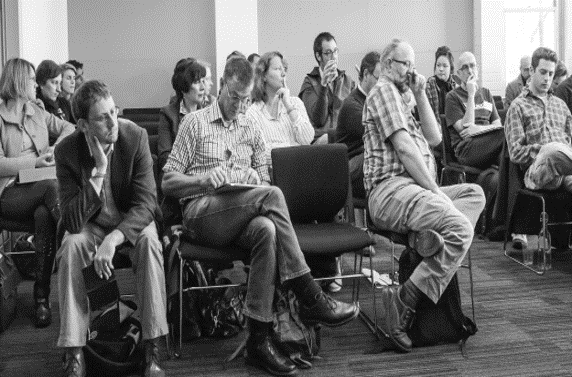
\includegraphics[height=.725\textheight]{figures/Archaeologists-standards.png}
        \caption{Archaeologists contemplate data standards (FAIMS Stocktaking, 2012)}
        \label{fig:figure7}
 \end{figure}
\end{frame}

%----------------------------------------------------------------------------------------

\begin{frame}{Context: the challenge of `small data'}
    `Long tail' research: most field data is small data \parencite{Borgman2015-rh}
    \begin{itemize}
        \item Smaller scale
        \item Diverse approaches
        \item Heterogeneous data
        \item Data and infrastructure emerge from fieldwork. 
        \item Relative lack of standards.
        \item Limited funding.
        \item Large(r) new data streams make everything harder.
        % \item Challenges associated with big(ger) data from photogrammetry, SfM, video, geophysics, etc., will exacerbate these problems.
    \end{itemize}
\end{frame}

%----------------------------------------------------------------------------------------


\begin{frame}{The data lifecycle}
 \begin{figure}[H]
    \centering
    \vspace{-0.5cm}
        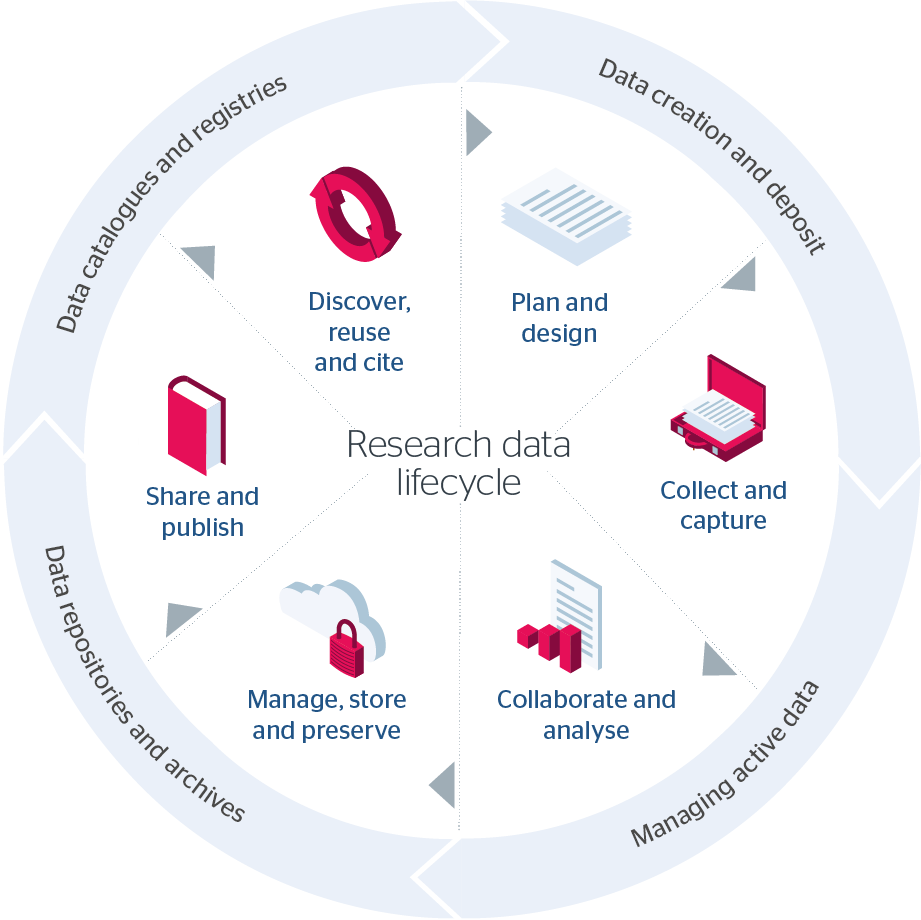
\includegraphics[height=.75\textheight]{figures/research-data-life-diagram.png}
        \caption{\cite{Jisc2018-gx} Image CC-BY-ND}
        \label{fig:figure9}
 \end{figure}
\end{frame}

%----------------------------------------------------------------------------------------


\begin{frame}{Infrastructure across the data lifecycle}
    Three main phases of the data lifecycle
    \begin{itemize}
        \item Publication (most mature)
        \item Processing and analysis (less mature) \parencite{Stewart_Lowndes2017-lj, Alveo2019-tk} .
        \item Capture (least mature and least supported by `normal' tools) \parencite{Bureau_of_Reclamation2017-xl}.
    \end{itemize}
\end{frame}

%----------------------------------------------------------------------------------------

\section{Nine years of FAIMS Mobile}

\begin{sectionframe} % Custom environment required for section slides
	\frametitle{Nine years of FAIMS Mobile}
	%\framesubtitle{Subtitle}

% 	Some section slide content

% 	This is on another line
\end{sectionframe}


%----------------------------------------------------------------------------------------

\begin{frame}{Research Specific}
 \begin{figure}[H]
    \centering
    \vspace{-0.5cm}
        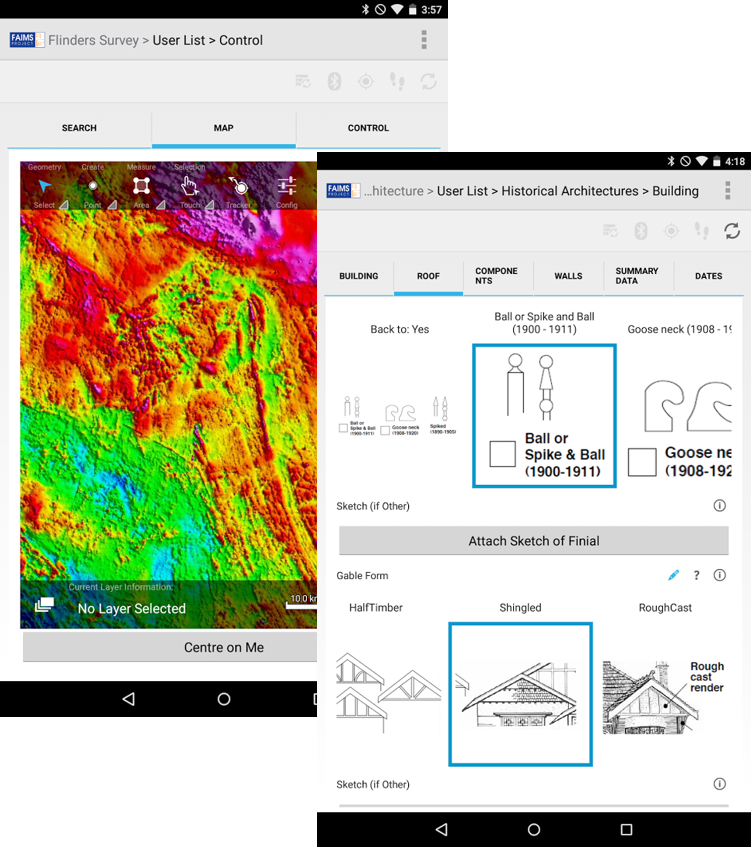
\includegraphics[height=.75\textheight]{figures/FAIMS-screenshots.png}
        \caption{FAIMS Mobile: GIS and `picture dictionaries'}
        \label{fig:FAIMS-mobile-screenshots}
 \end{figure}
\end{frame}

% %----------------------------------------------------------------------------------------

\begin{frame}{Key research-specific features}
	\begin{columns}[T]
		\begin{column}{0.45\textwidth}
        \begin{itemize}
            \item Customisable workflows.
            \item Offline capable.
            \item Complete data provenance / version history.
            \item Binds text, structured, geospatial, multimedia data.
            \item Mobile GIS with layers, raster and vector display, shape creation.
            \item Uses device and external sensors. 
            \item Multimedia file and metadata management.
        \end{itemize}
    \end{column}
	\begin{column}{0.45\textwidth}
        \begin{itemize}
            \item Validation and automation on device or server.
            \item Multilingual user-interface.
            \item Granular metadata: Notes and certainty for each field.
            \item Contextual help with images.
            \item Structured data can implement vocabularies / ontologies, LOD approaches.
            \item Data can be exported in a variety of formats, including custom exports.
        \end{itemize}
    \end{column}
\end{columns}
\end{frame}
%----------------------------------------------------------------------------------------

\begin{frame}{Generalised}
 \begin{figure}[H]
    \centering
        \vspace{-0.5cm}

        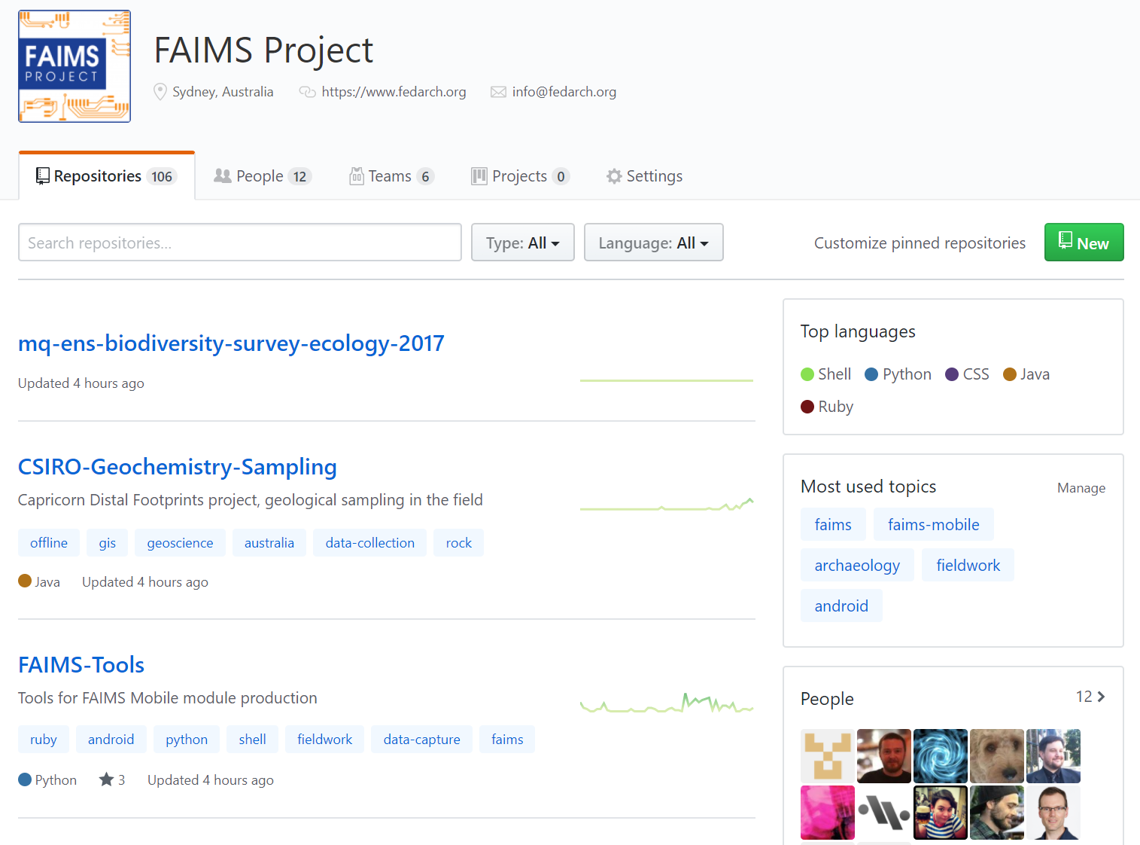
\includegraphics[height=.75\textheight]{figures/FAIMS-generalised.png}
        \caption{FAIMS Mobile customisations on GitHub}
        \label{fig:FAIMS-github}
 \end{figure}
\end{frame}
%----------------------------------------------------------------------------------------

\begin{frame}{Modular and federated}
 \begin{figure}[H]
    \centering
            \vspace{-0.5cm}

        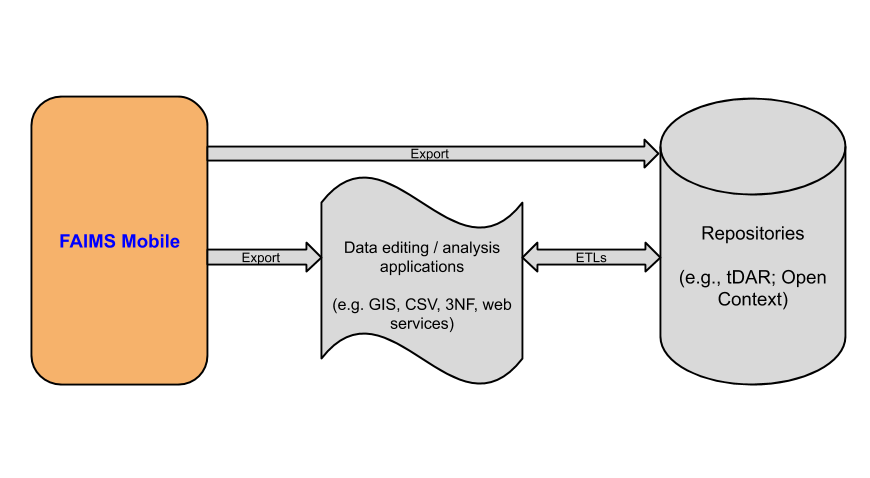
\includegraphics[height=.75\textheight]{figures/FAIMS-federation}
        \caption{FAIMS Mobile federation}
        \label{fig:FAIMS-federation}
 \end{figure}
\end{frame}
%----------------------------------------------------------------------------------------

\begin{frame}{Open Source}
 \begin{figure}[H]
    \centering
        
\includegraphics[width=.65\textwidth]{figures/asf_logo_url.png}
        
        \label{fig:FAIMS-github-OSS}
 \end{figure}
 
FAIMS Mobile v0.1-2.6 `core' code is licensed GPLv3; FAIMS 3.0 is licensed Apache 2.0; definition files are openly licensed (CC-BY); everything is on GitHub 

\end{frame}

%----------------------------------------------------------------------------------------

\begin{frame}{FAIMS by the numbers}
 \begin{itemize}
        \item \textbf{64 field data capture workflows customised}.
        \item \textbf{48 workflows confirmed deployed} to field at over \textbf{40 projects}.
        \item \textbf{100s of users} logged \textbf{10,000s hours} on the platform.
        \item Deployments took place in disciplines including \textbf{archaeology, geoscience, ecology, oral history, ecology, }and \textbf{linguistics}.
    \end{itemize}
\end{frame}
%----------------------------------------------------------------------------------------


\begin{frame}{Example deployments}
 \begin{itemize}
        \item Indigenous Foodways in the Cape York Peninsula (UNE, archaeology)
        \item Khirbet el-Rai Excavations, Israel (Macquarie, archaeology).
        \item Landscape Archaeology at Lake Mungo (LTU, archaeology)
        \item Excavation at the Boncuklu Höyük, Turkey (UQ, archaeology).
        \item Tao River Archaeological Project, China (Harvard, archaeology).
        \item Proyecto Arqueològico Zaña Colonial, Peru (Brown, archaeology).
        \item The Malawi Earlier-Middle Stone Age Project (Yale, archaeology).
        \item Avian Ecology in NSW (Macquarie, ecology)
        \item The Greek-Australian Historical Archive (UNSW, oral history).
        \item Key Pluridisciplinary Advances on African Multilingualism, Cameroon (SUNY Buffalo, linguistics).
        \item Capricorn Distal Footprints Project (CSIRO, geological sampling).

    \end{itemize}
\end{frame}
%----------------------------------------------------------------------------------------
\section{FAIMS 3.0}

\begin{sectionframe} % Custom environment required for section slides
	\frametitle{FAIMS 3.0}
	%\framesubtitle{Subtitle}

% 	Some section slide content

% 	This is on another line
\end{sectionframe}

%----------------------------------------------------------------------------------------

\begin{frame}{Where are we now?}
    \begin{itemize}
        \item FAIMS v2.6 is nearing end of its useful life.
        \item The FAIMS team did CSIRO ON Prime in 2016, completing 70+ interviews with clients / potential clients.
        \item A high-level technical plan for FAIMS v3.0 won a US design prize in 2017 \parencite{Bureau_of_Reclamation2017-xl}.
        \item ARDC Platforms announced a major co-investment in late 2019 to rebuild FAIMS using modern components.
    \end{itemize}
\end{frame}
%----------------------------------------------------------------------------------------


\begin{frame}{Opportunities and challenges}
    \begin{itemize}
        \item Useful research-specific features of FAIMS v2.6 to be retained.
        \item Android-only hindered uptake; cross-platform support required.
        \item Lack of self-service customisation / deployment hindered uptake.
        \item Users want to be able to edit data on the desktop or online, then have that data available for further editing in the field (data `round-trip' outside of the application).
        \item Users want more options for accessing / exporting data on-demand.
        \item Users want to be able to use the platform for sensitive data. 
        \item Improved scalability needed (application performance; server-to-server synchronisation)
        \item Enterprise features (orchestration, user management, reporting, branding, SSO, etc.) needed for eventual COSS \textbf{product} to support sustainability (underlying software \textbf{project} will remain OS).
    \end{itemize}
\end{frame}
%----------------------------------------------------------------------------------------

\begin{frame}{FAIMS 3.0 development approach}
Technical elaboration in 2020 produced an \href{https://zenodo.org/record/4616766}{Elaboration Report}; our approach includes:
    \begin{itemize}
        \item NODE.JS
        \item NoSQL datastore (Apache CouchDB / PouchDB)
        \item Progressive JS Single Page Application wrapped in Native code
for cross-platform support using Capacitor
        \item JSON Forms
        \item Javascript mapping library (LeafLet or OpenLayers)
        \item Plugin architecture
        \item APIs for data interactions

    \end{itemize}
\end{frame}
%----------------------------------------------------------------------------------------


\begin{frame}{FAIMS 3.0 development approach}
Other planned, but not yet elaborated, technical capabilities include:
    \begin{itemize}
        \item Web application to provide GUI to produce definition files
        \item 'Real' user management and security
        \item Interoperability with Cloudstor, EOSC nodes, ELNs, domain repositories (data `round-trip' export-modify-import)
        \item Device support (cameras, printers, instruments, etc.)
        \item Offline mapping
        \item Audio/video management
    \end{itemize}
\end{frame}

%----------------------------------------------------------------------------------------

\begin{frame}
    \frametitle{FAIMS 3.0 development progress}
    \framesubtitle{Development Progress}        
        \begin{itemize}
            \item \href{https://docs.google.com/document/d/13eTN8jhJa3Pgs9GOdo7r4jtIQcskNo7ikxJcBDBKHzw/edit}{Technical Elaboration Report} was approved in February. This established the proof-of-concept for FAIMS3. 
          \item \href{https://github.com/FAIMS/FAIMS3/releases/tag/v0.1.0-alpha}{Alpha prototype} was released on 11 June 2021.  
          \item Alpha prototype passed \href{https://doi.org/10.5281/zenodo.5030772}{user-acceptance testing} on 15 June 2021.
        \item FAIMS3 code has been licensed under the \href{https://www.apache.org/licenses/LICENSE-2.0}{Apache2} license, a Developer Contribution agreement is being applied to all code affirming the license. 
        \item The FAIMS3 repository is now public on \href{https://github.com/FAIMS/FAIMS3}{GitHub}.
        \item FAIMS3 Beta development commenced on 5 July 2021 and will conclude 1 November. 

    \end{itemize}



\end{frame} 
% %----------------------------------------------------------------------------------------


\begin{frame}{Thank you!}
PDF and source code for this presentation is available at: 
\texttt{https://github.com/FAIMS/FAIMS-intro/releases/tag/v1.0}.

FAIMS 3.0 project website: \texttt{https://faims.edu.au}.

FAIMS Project software, customisation library, and documentation can be found at:
\texttt{https://github.com/faims}.


This work is licensed under a Creative Commons Attribution 4.0 International License.

\end{frame}

% %----------------------------------------------------------------------------------------
% \section{References}

% \begin{sectionframe} % Custom environment required for section slides
% 	\frametitle{References}
% 	%\framesubtitle{Subtitle}
% % 	Some section slide content

% % 	This is on another line
% \end{sectionframe}



% %----------------------------------------------------------------------------------------
\begin{frame}[allowframebreaks]{References}

\printbibliography[heading=none, segment=1]
\end{frame}

\section{Extra: FAIMS research-specific features}

\begin{sectionframe} % Custom environment required for section slides
	\frametitle{Extra: FAIMS research-specific features}
	%\framesubtitle{Subtitle}

% 	Some section slide content

% 	This is on another line
\end{sectionframe}





%----------------------------------------------------------------------------------------
\begin{frame}[allowframebreaks]{Key research-specific features}
    \begin{itemize}
        \item Workflows and data schemata are deeply customisable.
        \item Customisation is achieved using relatively simple and human-readable XML documents separate from the ‘core’ software, supporting sharing, modification, and reuse via collaborative software development platforms like GitHub.
        \item Resulting mobile applications work offline.
        \item Automated bi-directional synchronisation using local or online server.
        \item A complete version history, with review and selective rollback, is provided for all data.
        \item Binds structured, geospatial, multimedia, and free text data in one record.
        \item A mobile GIS provides layer management and tools for the creation and editing of shapes.
        \item Connects to internal and external sensors (e.g., Bluetooth / USB devices).
        \item Externally captured multimedia (e.g., dSLR photos, audio recordings) can be connected to a record, then data contained in the associated record can be used to automatically rename connected multimedia files or write file metadata.
        \item Data validated on device and/or on server.
        \item Applications can be made multilingual using a standard and well-established localisation approach..
        \item Granular and contextualised metadata and certainty.
        \item Granular and contextualised help, including images, can be provided for all data entry fields.
        \item All data entry fields can be mapped to shared vocabularies, thesauri, or ontologies via embedded URIs, supporting Linked Open Data approaches.
        \item Data can be exported from the server in a variety of formats, or can be customised to a specific data target (e.g., JSON, relational database).
    \end{itemize}
\end{frame}
% %----------------------------------------------------------------------------------------

\section{Extra: The FAIMS approach in-depth}

\begin{sectionframe} % Custom environment required for section slides
	\frametitle{Extras: The FAIMS approach in-depth}
	%\framesubtitle{Subtitle}

% 	Some section slide content

% 	This is on another line
\end{sectionframe}


%----------------------------------------------------------------------------------------
\begin{frame}{Introduction to the FAIMS Project}
    \begin{itemize}
        \item The Field Acquired Information Management Systems (FAIMS) Project began in 2012 as a national Australian information infrastructure project in archaeology.
        \item Developed FAIMS Mobile for field data capture \parencite{Ballsun-Stanton2018-zd}.
        \item Use expanded beyond archaeology to geoscience, ecology, ethnography, linguistics, oral history.
        \item Has been customised for over 50 workflows at more than 30 projects. 
        \item Data and workflow modelling for customisations provided deep insights into field data capture and the infrastructure needed to support it.
    \end{itemize}
\end{frame}
%----------------------------------------------------------------------------------------
\begin{frame}{FAIMS Mobile software}
 \begin{figure}[H]
    \centering
    \vspace{-0.5cm}
        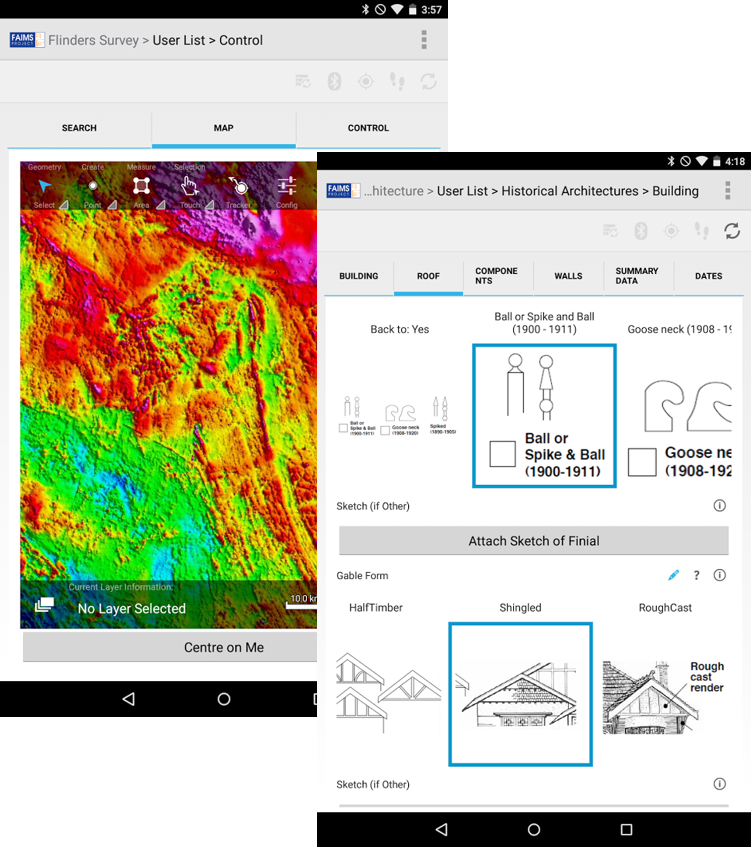
\includegraphics[height=.725\textheight]{figures/FAIMS-screenshots.png}
        \caption{FAIMS Mobile: GIS and `picture dictionaries'}
        \label{fig:figure10}
 \end{figure}
\end{frame}
%----------------------------------------------------------------------------------------
\begin{frame}{Field data capture infrastructure: a manifesto}
    \begin{itemize}
        \item Our domains deserve research-specific software.
        \item Diverse practices and limited resources require generalised software.
        \item Do one thing well with modular and federated software (but slice the pie thoughtfully).
        \item Open-source software supports open research and has other advantages (but is difficult to sustain). 
        \item Scope requirements carefully.
        \item Invest in outreach and engagement.
    \end{itemize}
\end{frame}
%----------------------------------------------------------------------------------------
\begin{frame}{Research specific}
    Field research needs (and deserves) research-specific software, contra \parencite{Roosevelt2015-kd}.
      \begin{itemize}
        \item Most commercial / mass-market software does not meet research needs.
        \item Risk of lock-in, unwelcome changes to features or business models, and product discontinuation.
    \end{itemize}
    \medskip{}
    Compare ecology: TERN, ALA, Biocollect, and associated research clouds \parencite{Tern2019-sp, Ala2019-by, Ala2019-cb}.
\end{frame}
%----------------------------------------------------------------------------------------
\begin{frame}{Generalised (not generic or bespoke)}
  Commercial software doesn't meet our needs, and bespoke development is too expensive and usually unsustainable.
      \begin{itemize}
        \item Generalised software can be deeply customised to accommodate our diverse data types, data models, workflows, etc.
        \item The code used to customise it describes the data model and workflow.
        \item Customisations can be published and re-deployed trivially.
        \item Can deliver research-grade software affordably.  
    \end{itemize}
    FAIMS Mobile cost perhaps 3x a single bespoke application, but has been customised 50x. Customisation cost is 1/10th bespoke, and still <1/2 even if `core' platform development costs are amortised across projects.
\end{frame}
%----------------------------------------------------------------------------------------
\begin{frame}{Generalised: customise using code}
 \begin{figure}[H]
    \centering
    \vspace{-0.5cm}
        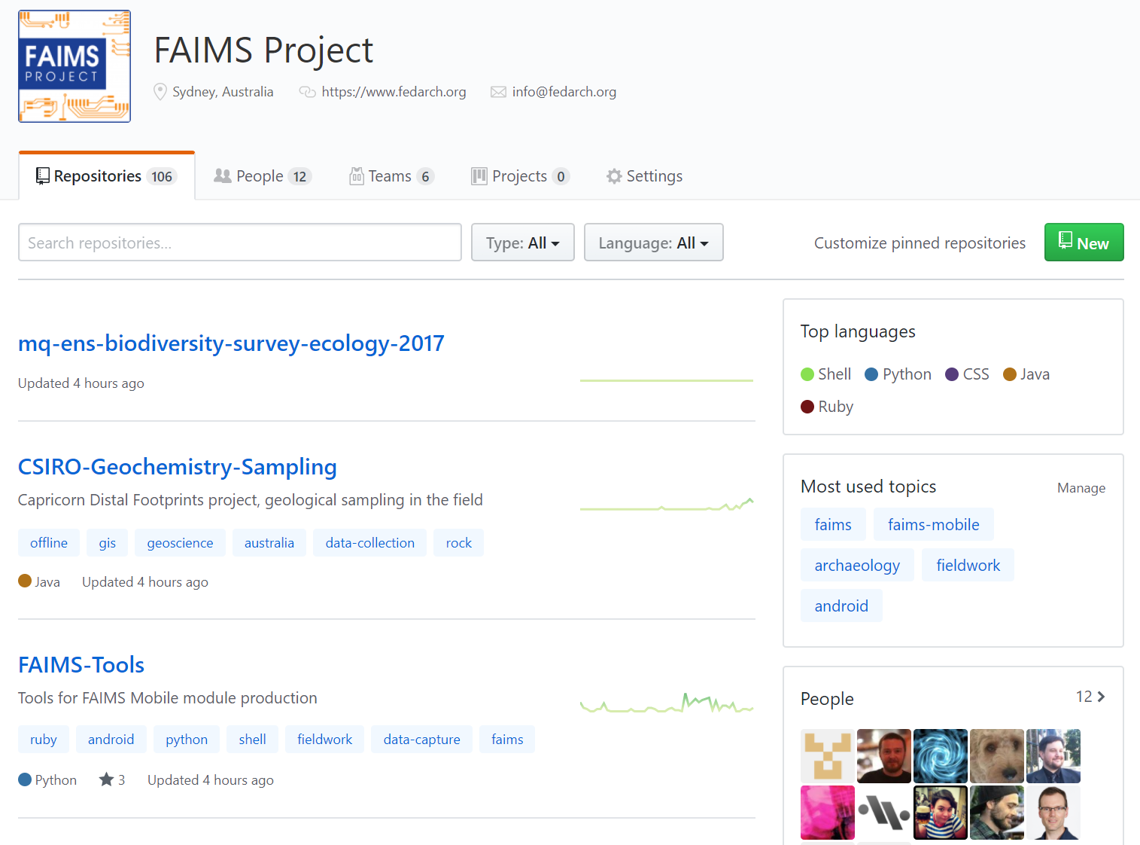
\includegraphics[height=.725\textheight]{figures/FAIMS-generalised.png}
        \caption{FAIMS Mobile customisations (XML files, mostly) on GitHub}
        \label{fig:figure11}
 \end{figure}
\end{frame}
%----------------------------------------------------------------------------------------
\begin{frame}{Modular and federated}
  \textbf{Do one thing well.}
      \begin{itemize}
        \item Identify other infrastructure in the domain and interoperate with it (via ETLs or APIs).
        \item It is better to divide by data-lifecycle phase rather than data type, since (1) our data is so integrated and (2) field data capture poses unique challenges.
    \end{itemize}
\end{frame}
%----------------------------------------------------------------------------------------
\begin{frame}{Modularise by data lifecycle phase}
 \begin{figure}[H]
    \centering
    \vspace{-0.5cm}
        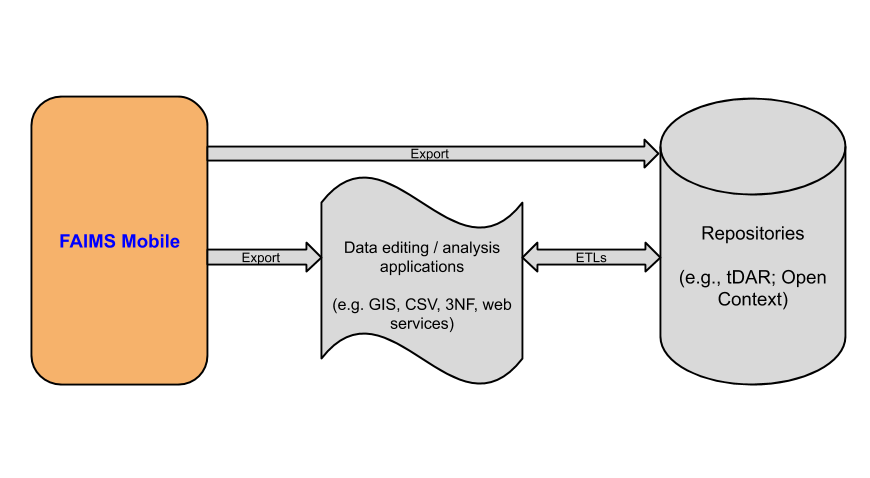
\includegraphics[height=.75\textheight]{figures/FAIMS-federation.png}
        \caption{FAIMS Mobile federation strategy}
        \label{fig:figure13}
 \end{figure}
\end{frame}
%----------------------------------------------------------------------------------------
\begin{frame}{Open source?}
  Open source has advantages but is difficult to sustain.
      \begin{itemize}
        \item Emerging open research principles strongly prefer OSS as opposed to proprietary ‘black boxes’.
        \item Transparency and reusability (esp. customisation code).
        \item Ability to hand off from one organisation to another (esp. `core' platform code).
        \item Ability to fork code prevents lock-in and mitigates unwelcome decisions by software developers.
        \item BUT OSS business models are hard to scale and rely on occasional injections of grant or institutional funding.
    \end{itemize}
\end{frame}
%----------------------------------------------------------------------------------------
\begin{frame}{Scope carefully}
  Talk to a wide range of potential users, seeking facts not opinions.
      \begin{itemize}
        \item Don’t ask researchers what they think, ask them what they have done - what software they have adopted and why, and what problems they have expended resources to solve. 
        \item ‘Lean startup’ methodology very useful, based around  testing of ideas through interviews with potential users \parencite{Strategyzer_AG2019-uu}.
        \item In our case, we over-invested in mobile GIS and under-invested in usability (especially a GUI for customisation).
    \end{itemize}
\end{frame}
%----------------------------------------------------------------------------------------
\begin{frame}{Spend on outreach and engagement}
  If you build it they will not come; people can't use technologies they don't know about.
      \begin{itemize}
        \item As per industry standards, dedicate at least 30\% of any information infrastructure budget to outreach and engagement (sales and marketing). 
        \item Typical academic outreach (journal articles, conference presentations, workshops, even booths at major conferences) are not enough.
    \end{itemize}
\end{frame}
%----------------------------------------------------------------------------------------
\section{Extras: Reports from the field}

\begin{sectionframe} % Custom environment required for section slides
	\frametitle{Extras: Reports from the field}
	%\framesubtitle{Subtitle}

% 	Some section slide content

% 	This is on another line
\end{sectionframe}

%----------------------------------------------------------------------------------------
\begin{frame}[allowframebreaks]{User feedback}
    \begin{itemize}
        \item ``The tablet app worked very well in the field and I would be keen to continue using it for subsequent sampling'' -- New Zealand Soil Geochemistry
        \item ``Being able to check in on everyone's work from my computer so easily is... revolutionary. Thank you for building such an amazing tool! …  I look forward to providing more details, but I already feel like I have 100\%{} better control over data quality, even compared to last year'' -- Proyecto Arquelogico de Zana Colonial
        \item ``The app has been such an incredible advantage in terms of workload, data quality, and a number of other data management issues with which archaeologists regularly have to deal. It readily links disparate data types that are otherwise stored separately – such as photographs, tabular logs, and context relationships.'' -- Malawi Early-Middle Stone Age Project
        \item ``I was really impressed with the approach FAIMS project has taken to the challenge of creating field data apps which can be very expensive. Our module was ready for testing after just one briefing.'' -- Streamwatch
        \item ``We’re back from the field and I cannot believe how well everything went. ... [T]he combination of the mobile lab, the sample ID/tracking and FAIMS application enabled us to average 5-6 minutes per sample site (crust, soil, rock and two plants)  in the field and about half that in the lab... Using the old school notepad and GPS approach this would have been 15 mins at best and a whole lot of misplaced photos and details, not to mention the additional hours entering the data in at night. We were able to identify missed sites as we went and completed the soils map (280 sites) and infill (36 sites) and analysis all in the 7 days. '' -- CSIRO Mineral Resources
    \end{itemize}
\end{frame}
\end{refsegment}
% %----------------------------------------------------------------------------------------
\section{Extras: FAIMS Publications}

\begin{sectionframe} % Custom environment required for section slides
	\frametitle{Extras: FAIMS Publications}
	%\framesubtitle{Subtitle}

% 	Some section slide content

% 	This is on another line
\end{sectionframe}
%----------------------------------------------------------------------------------------
\begin{frame}[allowframebreaks]{FAIMS Project bibliography}
\begin{refsegment}


\nocite{ballsun-stantonFAIMSMobileFlexible2018,rossBuildingBazaarEnhancing2015,rossCreatingEresearchTools2013a,rossIntroducingPreregistrationResearch2020,sobotkovaArbitraryOfflineData2015a,sobotkovaDeployingOfflineMultiuser2021,sobotkovaMeasureTwiceCut2016,sobotkovaSociotechnicalObstaclesArchaeological2018,thorneM436DistalFootprints2018,vanvalkenburghMobilizationMediationImplementing2018}

\printbibliography[heading=none, segment=2]

\end{refsegment}
\end{frame}
    

% %----------------------------------------------------------------------------------------
% \section{Text Examples}

% %----------------------------------------------------------------------------------------
% %	AUTOMATIC TEXT WRAPPING
% %----------------------------------------------------------------------------------------

% \begin{frame}[allowframebreaks] % 'allowframebreaks' allows automatic splitting across slides if the content is too long
% 	\frametitle{Automatic Text Wrapping}
% 	\framesubtitle{This text will automatically span across multiple slides\ldots}
	
% 	Lorem ipsum dolor sit amet, consectetur adipiscing elit. Praesent porttitor arcu luctus, imperdiet urna iaculis, mattis eros. Pellentesque iaculis odio vel nisl ullamcorper, nec faucibus ipsum molestie. Sed dictum nisl non aliquet porttitor.
	
% 	\bigskip
	
% 	Aliquam arcu turpis, ultrices sed luctus ac, vehicula id metus. Morbi eu feugiat velit, et tempus augue. Proin ac mattis tortor. Donec tincidunt, ante rhoncus luctus semper, arcu lorem lobortis justo, nec convallis ante quam quis lectus. Donec cursus maximus luctus. Vivamus lobortis eros et massa porta porttitor.

% 	\bigskip

% 	Fusce varius orci ac magna dapibus porttitor. In tempor leo a neque bibendum sollicitudin. Nulla pretium fermentum nisi, eget sodales magna facilisis eu. Praesent aliquet nulla ut bibendum lacinia.

% 	\bigskip

% 	Pellentesque lobortis justo enim, a condimentum massa tempor eu. Ut quis nulla a quam pretium eleifend nec eu nisl. Nam cursus porttitor eros, sed luctus ligula convallis quis. Nam convallis, ligula in auctor euismod, ligula mauris fringilla tellus, et egestas mauris odio eget diam. Praesent sodales in ipsum eu dictum.
% \end{frame}

% %----------------------------------------------------------------------------------------
% %	FONT OPTIONS
% %----------------------------------------------------------------------------------------

% \begin{frame}
% 	\frametitle{Font Options}

% 	Open Sans Light (default): Light, \textbf{Semibold}, \textit{LightItalic}, \textbf{\textit{SemiboldItalic}}

% 	\medskip

% 	Open Sans: {\OpenSans Regular, \textbf{Bold}, \textit{Italic}, \textbf{\textit{BoldItalic}}}

% 	\medskip

% 	Open Sans Condensed: {\OpenSansCondensed CondensedLight, \textbf{CondensedBold}, \textit{CondensedLightItalic}}

% 	\bigskip

% 	{\tiny tiny} {\scriptsize scriptsize} {\footnotesize footnotesize} {\small small} {\normalsize normalsize} {\large large} {\Large Large} {\LARGE LARGE} {\huge huge}
% \end{frame}

% %----------------------------------------------------------------------------------------
% %	SLIDE WITHOUT TITLE
% %----------------------------------------------------------------------------------------

% \begin{frame}
% 	Slides don't need to have titles.
% \end{frame}

% %----------------------------------------------------------------------------------------
% %	SLIDE WITHOUT TITLE WITH TITLE PADDING
% %----------------------------------------------------------------------------------------

% \begin{frame}
% 	\frametitle{\empty} % Empty so vertical whitespace is still added

% 	Slides can have empty titles, for alignment of content with slides with titles.
% \end{frame}

% %----------------------------------------------------------------------------------------
% %	EMPTY NO PADDING SLIDE
% %----------------------------------------------------------------------------------------

% \begin{frame}[plain]
% 	Slides can also be completely plain with no headers/footers and padding.

% 	\bigskip

% 	This is useful for large tables or figures.
% \end{frame}

% %----------------------------------------------------------------------------------------
% %	SECTION HIERARCHY
% %----------------------------------------------------------------------------------------

% \begin{frame}
% 	\frametitle{Heading Styling}

% 	\headinglevelone{Heading Level 1}

% 	Lorem ipsum dolor sit amet, consectetur adipiscing elit. Morbi eu feugiat velit, et tempus augue.
	
% 	\headingleveltwo{Heading Level 2}

% 	Praesent porttitor arcu luctus, imperdiet urna iaculis, mattis eros. Pellentesque iaculis odio vel nisl ullamcorper, nec faucibus ipsum molestie.
	
% 	\headinglevelthree{Heading Level 3}

% 	Sed dictum nisl non aliquet porttitor.
% \end{frame}

% %----------------------------------------------------------------------------------------

% \section{Blocks and column examples}

% %----------------------------------------------------------------------------------------
% %	COLUMNS
% %----------------------------------------------------------------------------------------

% \begin{frame}
% 	\frametitle{Using Columns}
% 	\framesubtitle{Two Columns}

% 	\begin{columns}[T]
% 		\begin{column}{0.45\textwidth}
% 			Lorem ipsum dolor sit amet, consectetur adipiscing elit. Morbi eu feugiat velit, et tempus augue. Praesent porttitor arcu luctus, imperdiet urna iaculis, mattis eros. Pellentesque iaculis odio vel nisl ullamcorper, nec faucibus ipsum molestie. Sed dictum nisl non aliquet porttitor.
% 		\end{column}
		
% 		\hfill

% 		\begin{column}{0.45\textwidth}
% 			Etiam vulputate arcu dignissim, finibus sem et, viverra nisl. Aenean luctus congue massa, ut laoreet metus ornare in. Nunc fermentum nisi imperdiet lectus tincidunt vestibulum at ac elit. Nulla mattis nisl eu malesuada suscipit.
% 		\end{column}
% 	\end{columns}
% \end{frame}

% %------------------------------------------------

% \begin{frame}
% 	\frametitle{Using Columns}
% 	\framesubtitle{Three Columns}

% 	\begin{columns}[T]
% 		\begin{column}{0.3\textwidth}
% 			Lorem ipsum dolor sit amet, consectetur adipiscing elit. Praesent porttitor arcu luctus, imperdiet urna iaculis, mattis eros. Pellentesque iaculis odio vel nisl ullamcorper.
% 		\end{column}

% 		\begin{column}{0.3\textwidth}
% 			
\includegraphics[width=\textwidth]{Faims-large.png}\\[6pt]
% 			Aenean tincidunt sodales massa, et hendrerit tellus mattis ac.
% 		\end{column}
		
% 		\begin{column}{0.3\textwidth}
% 			Aliquam arcu turpis, ultrices sed luctus ac, vehicula id metus. Morbi eu feugiat velit, et tempus augue. Proin ac mattis tortor. Donec tincidunt, ante rhoncus luctus semper.
% 		\end{column}
% 	\end{columns}
% \end{frame}

% %----------------------------------------------------------------------------------------
% %	BLOCKS
% %----------------------------------------------------------------------------------------

% \begin{frame}
% 	\frametitle{Using Beamer Blocks}

% 	\begin{columns}[T]
% 		\begin{column}{0.3\textwidth}
% 			\begin{block}{Block Title}
% 				Aliquam arcu neque, ornare in, ullamcorper quis, commodo eu, libero. Maecenas sapien libero, lobortis in, sodales eget, dui.
% 			\end{block}
% 		\end{column}

% 		\begin{column}{0.3\textwidth}
% 			\begin{block}{\centering Centered Block Title}
% 				Aliquam arcu neque, ornare in, ullamcorper quis, commodo eu, libero. Maecenas sapien libero, lobortis in, sodales eget, dui.
% 			\end{block}
% 		\end{column}

% 		\begin{column}{0.3\textwidth}
% 			\begin{block}{\vspace{-\baselineskip}}
% 				Aliquam arcu neque, ornare in, ullamcorper quis, commodo eu, libero. Maecenas sapien libero, lobortis in, sodales eget, dui.
% 			\end{block}
% 		\end{column}
% 	\end{columns}
% \end{frame}

% %----------------------------------------------------------------------------------------
% %	ALERT BLOCK
% %----------------------------------------------------------------------------------------

% \begin{frame}
% 	\frametitle{Alert Blocks}
% 	\framesubtitle{Useful for Important Information}

% 	\begin{columns}[T]
% 		\begin{column}{0.45\textwidth}
% 			Etiam vulputate arcu dignissim, finibus sem et, viverra nisl. Aenean luctus congue massa, ut laoreet metus ornare in. Nunc fermentum nisi imperdiet lectus tincidunt vestibulum at ac elit. Nulla mattis nisl eu malesuada suscipit.
% 		\end{column}
		
% 		\hfill

% 		\begin{column}{0.45\textwidth}
% 			\vspace*{-\baselineskip} % For vertical alignment with the text
% 			\begin{alertblock}{Alert Block Title}
% 				Suspendisse vitae elit. Aliquam arcu neque, ornare in, ullamcorper quis, commodo eu, libero. Fusce sagittis erat at erat tristique mollis. Maecenas sapien libero, molestie et, lobortis in, sodales eget, dui.
% 			\end{alertblock}
% 		\end{column}
% 	\end{columns}
% \end{frame}

% %----------------------------------------------------------------------------------------
% %	EXAMPLE BLOCK
% %----------------------------------------------------------------------------------------

% \begin{frame}
% 	\frametitle{Example Blocks}

% 	\begin{columns}[T]
% 		\begin{column}{0.6\textwidth}
% 			\vspace*{-\baselineskip} % For vertical alignment with the text
% 			\begin{exampleblock}{Example Block Title}
% 				Suspendisse vitae elit. Aliquam arcu neque, ornare in, ullamcorper quis, commodo eu, libero. Fusce sagittis erat at erat tristique mollis. Maecenas sapien libero, molestie et, lobortis in, sodales eget, dui. Morbi ultrices rutrum lorem. Nam elementum ullamcorper leo. Morbi dui. Aliquam sagittis. Nunc placerat. Pellentesque tristique sodales est.
% 			\end{exampleblock}
% 		\end{column}

% 		\hfill

% 		\begin{column}{0.3\textwidth}
% 			Etiam vulputate arcu dignissim, finibus sem et, viverra nisl. Aenean luctus congue massa, ut laoreet metus ornare in. Nunc fermentum nisi imperdiet lectus tincidunt vestibulum at ac elit.
% 		\end{column}
% 	\end{columns}
% \end{frame}

% %----------------------------------------------------------------------------------------

% \section{Slide element examples}

% %----------------------------------------------------------------------------------------
% %	LISTS
% %----------------------------------------------------------------------------------------

% \begin{frame}
% 	\frametitle{Lists}

% 	\begin{enumerate}
% 		\item First numbered item
% 		\begin{enumerate}
% 			\item First indented numbered item
% 			\item Second indented numbered item
% 			\begin{enumerate}
% 				\item First second-level indented numbered item
% 			\end{enumerate}
% 		\end{enumerate}
% 		\item Second numbered item
% 	\end{enumerate}

% 	\rule{\textwidth}{0.25pt}

% 	\begin{itemize}
% 		\item First bullet point item
% 		\begin{itemize}
% 			\item First indented bullet point item
% 			\item Second indented bullet point item
% 			\begin{itemize}
% 				\item First second-level indented bullet point item
% 			\end{itemize}
% 		\end{itemize}
% 		\item Second bullet point item
% 	\end{itemize}
% \end{frame}

% %----------------------------------------------------------------------------------------
% %	TABLE
% %----------------------------------------------------------------------------------------

% \begin{frame}
% 	\frametitle{Table}
% 	\framesubtitle{Displaying Data}

% 	\begin{table}
% 		\centering % Center the table in the slide
% 		\begin{tabular}{L{0.18\textwidth} R{0.11\textwidth} R{0.11\textwidth}}
% 			\toprule
% 			\textit{Per 50g} & \textbf{Pork} & \textbf{Soy} \\
% 			\midrule
% 			Energy & 760kJ & 538kJ\\
% 			Protein & 7.0g & 9.3g\\
% 			Carbohydrate & 0.0g & 4.9g\\
% 			Fat & 16.8g & 9.1g\\
% 			Sodium & 0.4g & 0.4g\\
% 			Fibre & 0.0g & 1.4g\\
% 			\bottomrule
% 		\end{tabular}
% 	\end{table}
% \end{frame}

% %----------------------------------------------------------------------------------------
% %	IMAGE
% %----------------------------------------------------------------------------------------

% \begin{frame}
% 	\frametitle{Image/Figure}
% 	\framesubtitle{Including a Centered Image, Such As of a Graphical Figure}

% 	\begin{center}
% 		
\includegraphics[width=0.5\textwidth]{Faims-large.png}
% 	\end{center}
% \end{frame}

% %----------------------------------------------------------------------------------------
% %	EQUATION
% %----------------------------------------------------------------------------------------

% \begin{frame}
% 	\frametitle{Equation}

% 	\begin{equation}
% 		\cos^3 \theta =\frac{1}{4}\cos\theta+\frac{3}{4}\cos 3\theta
% 	\end{equation}
% \end{frame}

% %----------------------------------------------------------------------------------------
% %	REFERENCES
% %----------------------------------------------------------------------------------------

% \begin{frame}
% 	\frametitle{Referencing}

% 	This statement requires citation \autocite{Smith:2019qr}. This statement requires multiple citations \autocite{Smith:2019qr, Smith:2021jd}. This statement contains an in-text citation, reminiscent of that in \textcite{Smith:2021jd}.
% \end{frame}

% %----------------------------------------------------------------------------------------

% \section{Custom slides}

% %----------------------------------------------------------------------------------------
% %	IMAGE SLIDE
% %----------------------------------------------------------------------------------------

% \imageslide{Monasterio_Khor_Virap_Armenia.jpg} % Image automatically takes up the full width of the slide, crop it if it's too tall

% %----------------------------------------------------------------------------------------
% %	BIG NUMBER SLIDE
% %----------------------------------------------------------------------------------------

% \begin{bignumframe}{20\%} % Big number slide, first argument should be the big number
% 	Lorem ipsum dolor sit amet, consectetur adipiscing elit. Praesent porttitor arcu luctus, imperdiet urna iaculis, mattis eros.

% 	\bigskip

% 	\begin{itemize}
% 		\item Etiam vulputate arcu dignissim, finibus sem et, viverra nisl.
% 		\item Aenean luctus congue massa, ut laoreet metus ornare in.
% 	\end{itemize}
% \end{bignumframe}

% %----------------------------------------------------------------------------------------
% %	REFERENCE LIST
% %----------------------------------------------------------------------------------------

% \begin{frame}[allowframebreaks] % 'allowframebreaks' allows automatic splitting across slides if the content is too long
% 	\frametitle{Bibliography}

% 	\printbibliography[heading=none]
% \end{frame}

% %----------------------------------------------------------------------------------------

% % Long section title example
% \section{Lorem ipsum dolor sit amet, consectetur adipiscing elit. Morbi eu feugiat velit, et tempus augue.}

%----------------------------------------------------------------------------------------
%	CLOSING SLIDE
%----------------------------------------------------------------------------------------

\closingslide % Output closing slide, automatically populated with a background image

%----------------------------------------------------------------------------------------

\end{document}
